% !TeX root = main.tex

\section{GEE 实现}

基于 GEE 平台, 下文将给出计算清华大学校园内 VI 时空分布的方法, 整体的处理流程如 \cref{fig:flow} 所示.
完整的 GEE 源码见 \cref{app:code}.

\begin{figure}[htbp]
  \centering
  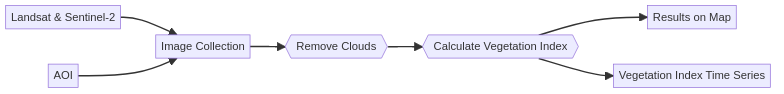
\includegraphics[width=\linewidth]{assets/flow-chart.png}
  \caption{Methodology}
  \label{fig:flow}
\end{figure}

\subsection{预处理数据}

不同版本的 Landsat 数据集覆盖的时间范围不同, 通过将 Landsat 4-9 的数据进行整合, 影像数据的时间跨度能够大幅延长.

\begin{minted}{js}
// * Image Collection > Landsat
function SRImageCollection(duration, cutout, threshold) {
  // image collections are imported using the "imp" file
  var L9sr = imp.ColeccionLandsatSR(duration, "LC09", cutout, threshold);
  var L8sr = imp.ColeccionLandsatSR(duration, "LC08", cutout, threshold);
  var L7sr = imp.ColeccionLandsatSR(duration, "LE07", cutout, threshold);
  var L5sr = imp.ColeccionLandsatSR(duration, "LT05", cutout, threshold);
  var L4sr = imp.ColeccionLandsatSR(duration, "LT04", cutout, threshold);
  // ETM and ETM+ data are spectral fit to OLI and OLI-2
  var L7a = L7sr.map(imp.TMaOLI);
  var L5a = L5sr.map(imp.TMaOLI);
  var L4a = L4sr.map(imp.TMaOLI);
  // join collections
  var series = L9sr.merge(L8sr)
    .merge(L7a)
    .merge(L5a)
    .merge(L4a)
    .sort("system:time_start");
  return series;
}
\end{minted}

除了 Landsat 外, Sentinel-2 数据集也提供公开访问.
为了保证数据的有效性, 云量过高的数据需要被剔除, 本文选取 $\mathtt{clouds} = \SI{30}{\percent}$ 为阈值.

\begin{minted}{js}
// * Image Collection > Landsat & Sentinel-2
function CollectionImageBoth(duration, cutout, threshold) {
  // function for Landsat images with spectral adjustment
  var L8Set = SRImageCollection(duration, cutout, threshold);
  // Sentinel-2
  var S2sr = imp.ColeccionImagenSentinelSR(duration, cutout, threshold);
  // spectral matching of Sentinel-2 to Landsat
  var S2a = S2sr.map(imp.MSIaOLI);
  var series = S2a.merge(L8Set).sort("system:time_start");
  return series;
}

// the collection is imported
var S2B = CollectionImageBoth(duration, table, clouds);
\end{minted}

\subsection{计算植被指数 (VI)}

基于 Jiménez \cite{jimenez-jimenez_vical_2022} 的工作, 我们很容易在预处理后的数据集上计算 VI.

\begin{minted}{js}
// * Vegetation indices
// Normalized Difference Vegetation Index --- NDVI
var index_name = "NDVI";
var vis = ee.ImageCollection(S2B.map(imp2[index_name]));
\end{minted}

\subsection{导出计算结果}

计算完成后, 可以将计算结果中某一时刻的 VI, 例如可用数据集中最早的时刻, 作为新的图层直观地显示在 GEE 的地图中进行分析.

\begin{minted}{js}
// NDVI from the first image in the collection
var vi = vis.first();
// color palette where 'st' file is used
var viVis = { min: 0, max: 1, palette: st.paletaIV };
Map.addLayer(vi.clip(table), viVis, index_name); // index
// the map is centered to the area
Map.centerObject(table, 15);
\end{minted}

除此之外, 不同时段的 VI 数据也可以通过 \verb|ui.Chart| 按时间序列导出下载.

\begin{minted}{js}
// * Time Series
var filtered = boundary;
var reducers = ee.Reducer.mean().combine({
  reducer2: ee.Reducer.stdDev(),
  sharedInputs: true,
});
var chart = ui.Chart.image.series(vis, filtered, reducers, 10).setOptions({
  title: "Vegetation Index Time Series",
  hAxis: { title: "Date", format: "yyyy-MM" },
  vAxis: { title: index_name },
});
print(chart);
\end{minted}
